\chapter{Technical overview}
In this chapter we will elaborate on how the application for \textit{Archipelago} is constructed, the structure of the app and the scenes contained within it and how they function. After that, we will go into more details on the UI elements and user interaction, as well as how the users can interact with and move around the viewport to better get an overlook of the map, and this will lead on to the world map itself with its layout and how it is constructed. This will then be followed by a detailed description of how the PCG algorithms work and how the events with its options, outcomes and flavour is constructed. In the end of this chapter we will go through the app in action from start to end and how it is utilized together with its features.

\section{App structure}
This section details the overall structure of the app.
First the scenes in their structure in the game and later the UI and additional elements.

\subsection{Scenes}
\label{sec:scen}
This section is dedicated to the overview of the technical relation between the different scenes and their individual purpose. Each scene will be detailed in each of the following subsections going from the first scene in the app, to the last scene.
The transitions between the different scenes can be seen in the overview presented by figure \ref{fig:appState}. The names on the transitions are related to the button presses which initiate them. 
The diagram does not show any of the actions which transition to the same state.

\begin{figure}[!ht]
    \centering
    \includegraphics[scale=0.5]{Images/StateDiagram.png}
    \caption{The overview of the scenes in the application and their linkage. The diagram shows each of the actions which change to other scenes.}
    \label{fig:appState}
\end{figure}

\subsubsection{StartMenu}
As the game is started, you immediately enter the start screen. This is a simple scene containing only the button that says "Start Game". The purpose behind this scene is to let the users be able to chose when they want to start the game, so that they are not necessarily overpowered by the rules of the game (board game part) and the visuals of the app itself when started.

Furthermore, as this scene is loaded, the preliminaries to the world generation and the loading of required data from XML files is handled. This minor loading, takes some of the load of the rest of the program, giving an overall smoother experience.
This includes the general l-system structure, which is run in the start menu, the loading of board game pieces, and the loading of the different factions in the game.

As soon as the "Start Game" button is clicked, the app will initialize the contents of the world, and present it to the user within the next scene, which is the WorldScene.

\subsubsection{WorldScene}
\label{sec:worldscene}
This is the main layout of the world. It contains all the locations that the players can travel to, and shows them where they are, where they have been, and where they have to go.

When you first see this part of the program, you will notice that it has floating islands with rings around them, as well as a flying castle. The castle is the piece the players control, and it is what the board is representing in the physical part of the game.
At first glance, you might not see all of the map and all the different islands you can travel to, but by simply zooming out, the players are able to get a better view of the entire map layout, and from there, they can plan their chosen way. There is also a little arrow in the lower right corner of the screen, which always will point towards the goal-island. 
In figure \ref{fig:worldSc} you can see the scene which meets you once the scene is loaded.

\begin{figure}[!ht]
    \centering
    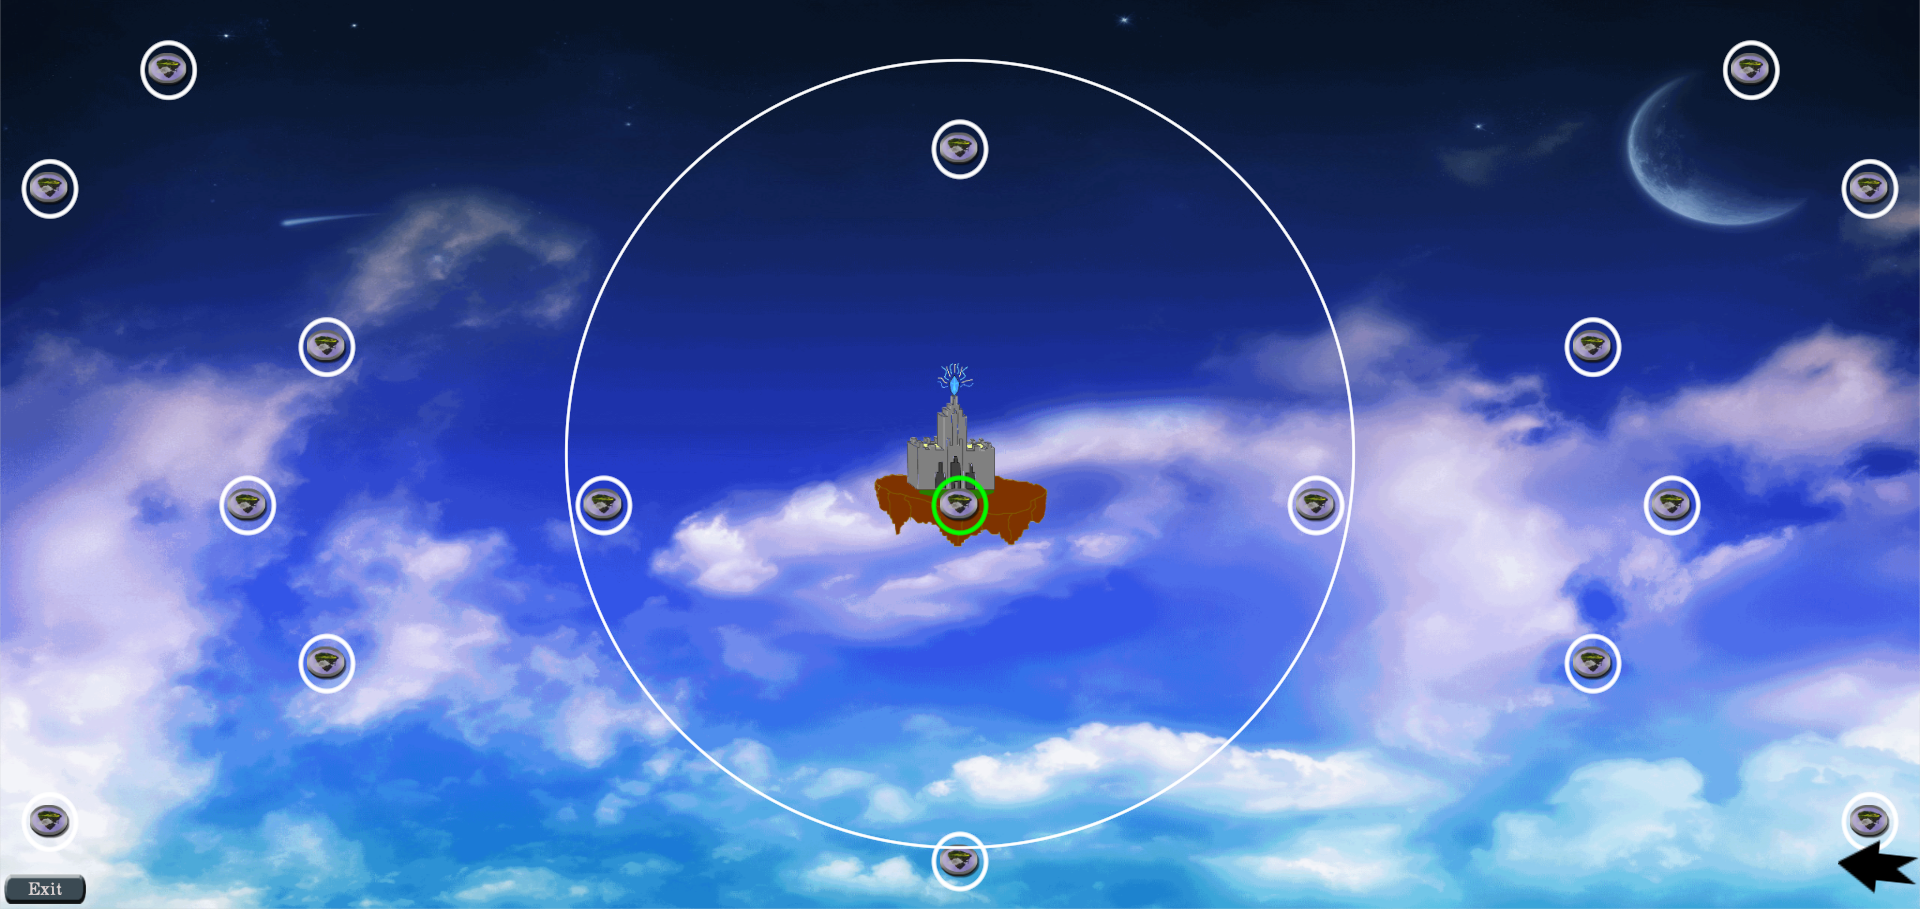
\includegraphics[scale=0.3]{Images/WorldScene.png}
    \caption{The WorldScene as seen on the PC version of the App. In the center the player token is represented as a floating castle. Also seen in the center is the green node, denoted as the starting node. In the lower right corner is the arrow pointing towards the goal node. The outer white ring indicates the maximum travelling distance of the players.}
    \label{fig:worldSc}
\end{figure}

As seen in the figure, there is a large white ring centered on the castle that the players control. This ring is indicating the range that the castle can travel in one turn of the game. Any islands that are within this ring, are available to be travelled to.
When travelling from one island to another, the ring around the island you arrived at will change color (from the initial white color). This signifies to the players that they have already been to that island and therefore do not necessarily have to go back to that place again unless they choose to do so.

When you click an island on the map, you will be faced with a pop-up box. This box is containing the name of the island, and a piece of text that somewhat describes it; flavour text. The box then has 2 buttons, or choices, either "exit" or "travel". If you exit, the box is closed, and you are free to choose another island to travel to. If you click travel, however, your castle will be moved towards that chosen island and stop once it reaches it. 
Once the castle has reached the island and the collider on the object is triggered, the app will move on to the NodeScene, where the island that you travelled to will be represented.

\subsubsection{NodeScene}
\label{sec:nodeScene}
The NodeScene is probably best known as the "island scene" or "event scene", because this is the scene where all the events take place, and it is the main place where the players will have to interact with each other in order to choose their wanted event.

Once this scene is loaded the events for the given island and the locations on it, are generated. The events uses the information from the world node in order to create the events. The reason the event generation to be moved to this location, were to limit the computing power required to initialize the world node. 

\begin{figure}[!ht]
    \centering
    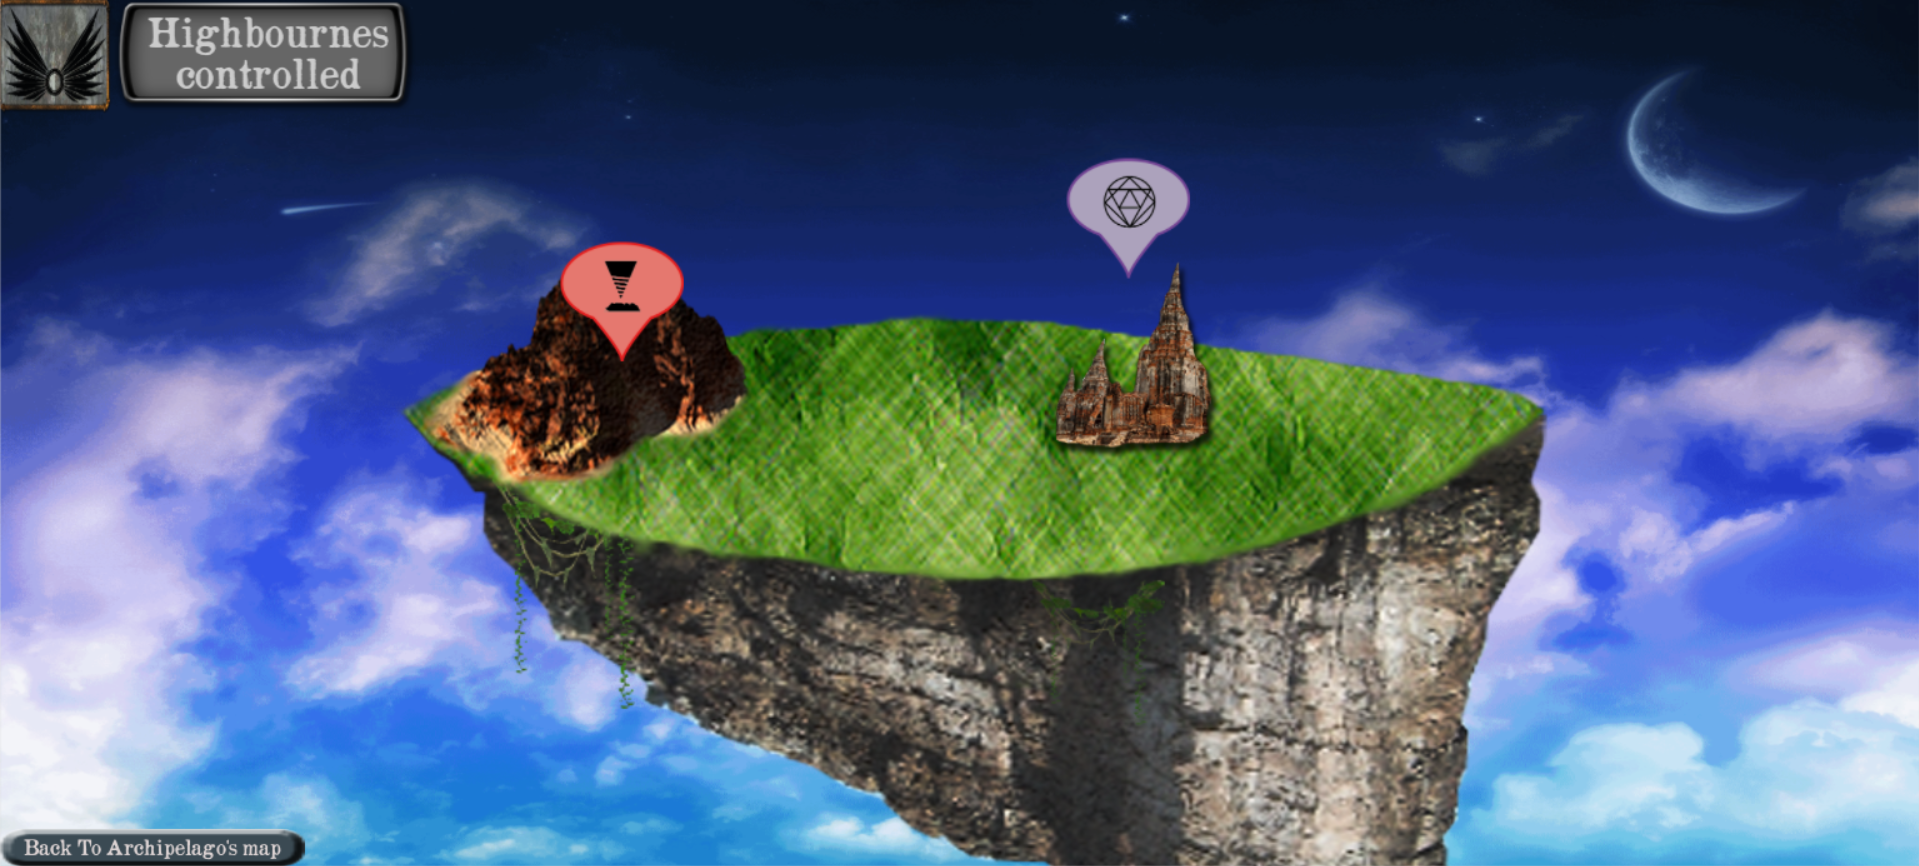
\includegraphics[width=\textwidth]{Images/NodeScene.png}
    \caption{The node scene as seen on the computer version of the app. In the center is the island, with two locations situated on it, a mine and a ruin. In the top left corner, it can be seen that the island is controlled by the Highbourne.}
    \label{fig:nodescene}
\end{figure}

In figure \ref{fig:nodescene} you can see one of the configurations that the island can have on generation. The island has two locations for the players to explore, a mine and a ruin. 
Each time an island is generated, it always comes with two locations for the players to visit, one for gathering and one for research. The gathering event will have a red icon with a drill on it hovering above the given location, whilst the research event will have will have a blue icon with a alchemical symbol.
Research events usually yield more alchemy points, whereas the gathering event has their basis in building materials.

Each island also have a general faction which in charge of all the locations on the island. Their icon and their affiliated symbol is located in the top left corner. From this the players are able to easily identify whether they have arrived at a location where they have allies or enemies, and from that conclude whether their events are going to have a higher chance of success with better outcomes, allied faction, or if there is going to be a higher chance of failure with worse outcomes, enemy faction.
The faction is also displayed on the travel panel presented in the WorldScene, giving the players the opportunity to choose which factions they wish to interact with.

\begin{figure}[!ht]
    \centering
    \begin{subfigure}[b]{\textwidth}
        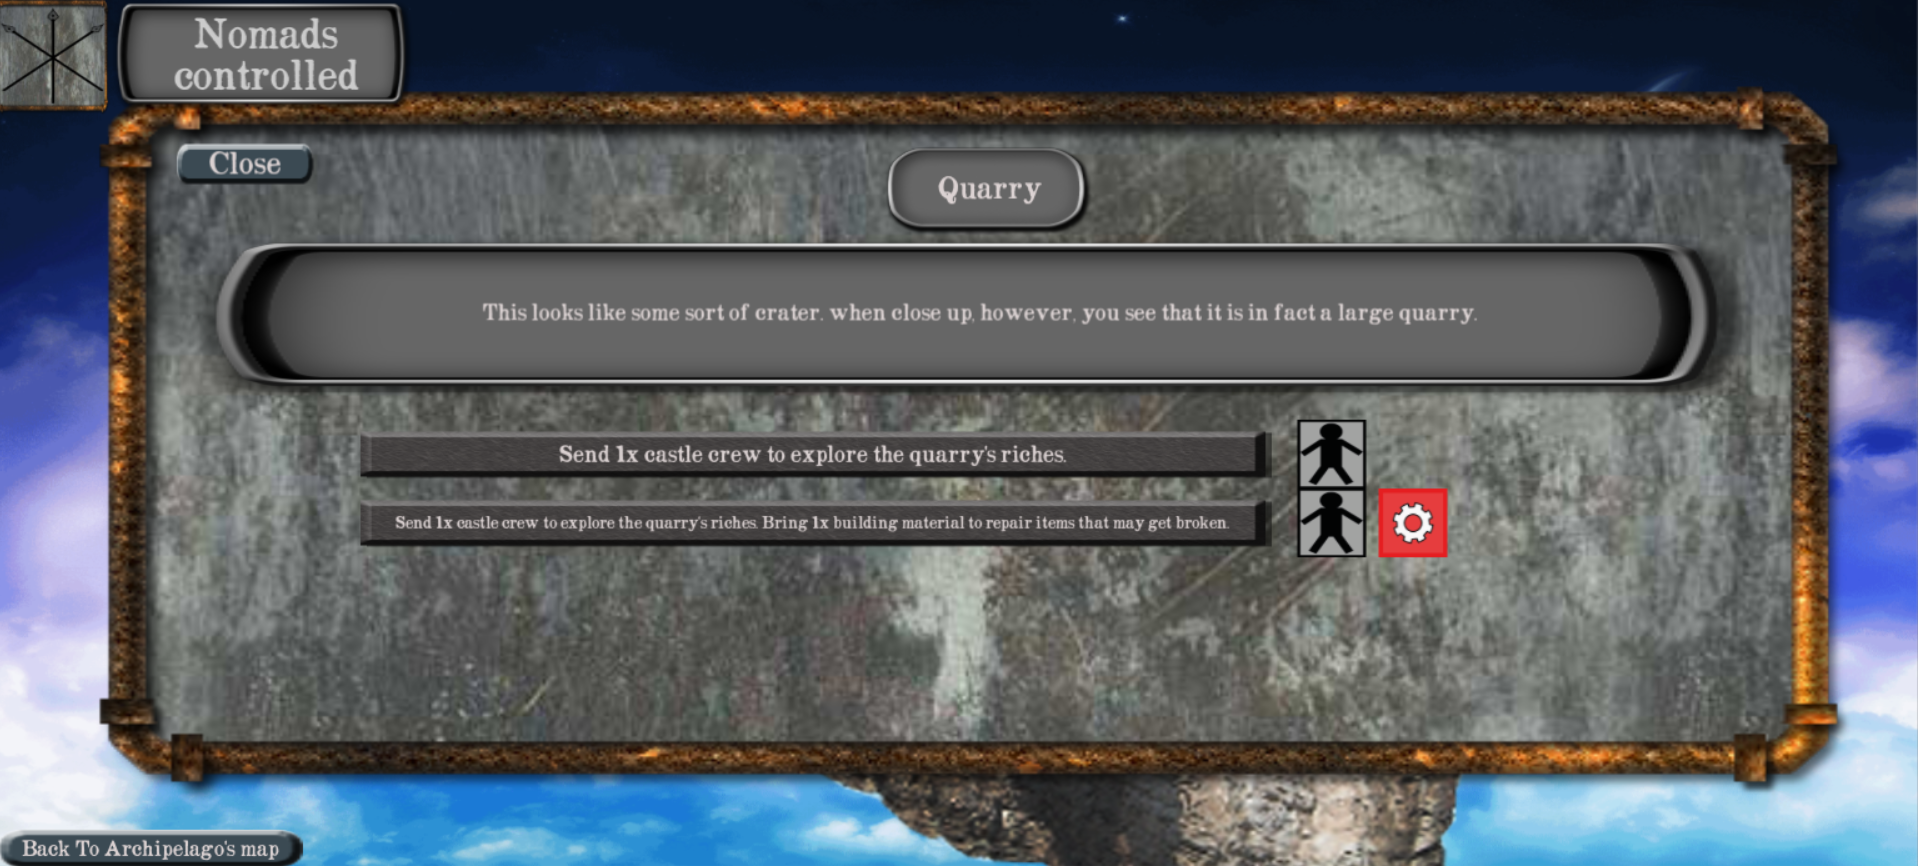
\includegraphics[width=\textwidth]{Images/EventPanel.png}
        \caption{This is the panel related to the event of a location the players have chosen to explore. In the top of the panel there is the name of the location which the players are exploring.
       In the middle of the panel is the buttons which resolves the event, with the requirements of the event represented as images next to the button.
        Above the buttons is a short description of the event, referred to as flavour text. If the panel was opened by mistake, the panel can be closed using the associated button in the top left corner. }
        \label{fig:evepan}
    \end{subfigure}
    \begin{subfigure}[b]{\textwidth}
        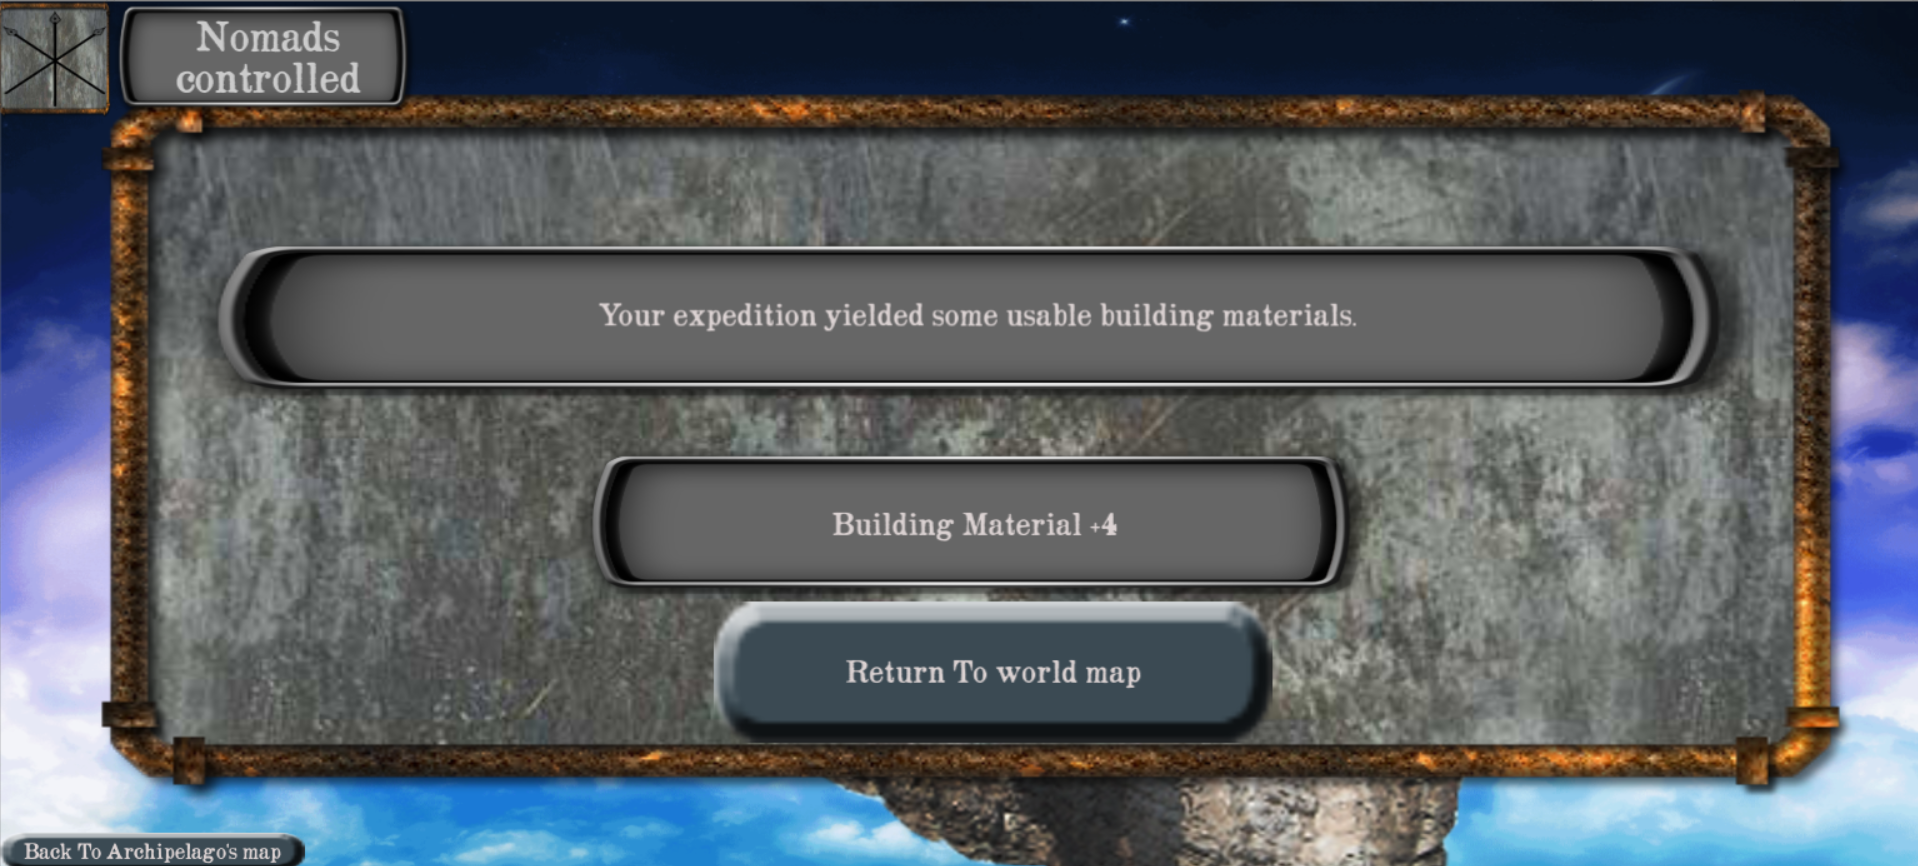
\includegraphics[width=\textwidth]{Images/EventResolution.png}
        \caption{The panel related to the resolution of the events. The panel comes with a short flavour text about what has transpired, followed by a list of the gameplay objects which have been changed in the event. The panel can be closed by clicking the return to world map, ending the scene and initializing the WorldScene.}
        \label{fig:everes}
    \end{subfigure}
    \caption{Images of the different panel in the event execution.}
    \label{fig:eventPans}
\end{figure}

Once an area of the island has been clicked, a confirm box will be shown where the player will have to confirm that this is the area they want to explore. 

Once the explore button is clicked, the panel in figure \ref{fig:evepan} will appear. 
This panel displays the location you have chosen to explore along with some flavour text about the location. 
The panel will come with either 2 or 3 options, in the example there is only two, represented as buttons below the flavour text. 
Each option have one or more requirements, which a both included in the flavour text on the button and displayed as images next to it. These requirements are the resources the players must commit in order to resolve the event. 
E.g. "Send 1x castle crew to explore the quarry's riches. Bring 1x building material along to repair items that may get broken.", tells the players that they need 1 castle crew and 1 building material to commit to this option.

Once you have selected an option, the panel will shift to the resolution panel as seen in figure \ref{fig:everes}. The event is concluded and the players is presented with the results of their choice. The result comes in the form of a flavour text describing what happened, and a list of either rewards or penalties.
Once the players close the resolution panel, they will return back to the WorldScene, ready to move on to the next island.

\subsubsection{ScoreScene}
Upon reaching the final island in the WorldScene, the one island with the blue ring around it and that the arrow, that was mentioned earlier, is pointing towards, the game ends. 
What happens then is that all the data is cleared from the app, the WorldScene shifts to the ScoreScene, and the players are presented with an end text that basically tells them that they reached the goal. This scene also includes a button that takes the players back to the StartMenu where they can play another game if they so choose.

\subsection{Buttons and Raycasting on images}
The players main source of interaction is via the use of buttons and images. The buttons that can be found on the main screen, on various events and dialog boxes, all have their own respective functionalities connected with them. One button might close a box, another might start the game, each button have specific actions that they perform, and what they do or how they affect the gameplay, is represented on them either via specific text, flavour text or icons.
The images and icons are a bit more tricky, especially for the players, as they do not necessarily signify to them that they can be interacted with, unlike the buttons which most people instinctively know does something.
By programming itself, an image is just an image. It has no function attached to it, and does not do anything specific other than portraying a picture. So in order to make the images \textit{clickable} you have to introduce raycasting.

Raycasting is when you create a line from one point to another, and in this case the only logical way to raycast to the images, was to make the initial start point be wherever the user touch the screen. So when the screen is touched, and the initial position is set, a ray will be made from that point and go \textit{into} the screen (the z direction). By doing this, we can calculate if at any point of the ray, it touches an image that we want to give functionality. If this is the case and say that an exploration location is colliding with the ray, the application will then know to execute the functionalities that that images is holding. In the case of a location being clicked, an event box will appear and the players can continue with the game, and explore on.

In the next section, the UI Elements section, you will be introduced to all the remaining elements that is used in the digital part of the game.

\subsection{UI elements}
In this section, we will go through all the different UI elements within the app and explain in more detail their purpose and how they work.

\subsubsection{Boxes}

There are a number of different boxes that will appear over the course of a game session with this app. By "boxes" we refer to the dialog boxes that pop up when interacting with different elements of the application itself, e.g. an event popping up when interacting with an island.
The purpose of each box on a high level, is to convey information to the players, be it information about the location that they are travelling to, or the results of an event they have just completed.
Each box has it's own purpose, but as just stated, the main purpose is to convey information. The first box that appears when interacting with the app, is the "travel confirmation" box. This box tells a little information about the island that the player wishes to travel to, like the name of the island, and a few lines of flavour text that goes with said name. It also contains two buttons; one for accepting the travel location, and another one cancelling.
Once you have travelled to a location the next box will appear when the region the players want to explore is clicked. This box, like the one before, has a name (the location type like "mine") and a text field for the flavour about that mine. Again there is a button for accepting, and one for declining. 

Next up, you have the event box. This is the main box of the game, one might say. It contains a text field where the procedurally generated flavour text is displayed, along with 2 or 3 buttons that has the options for completion that the players may choose from. 
Once an option has been chosen, the application loads the result box. This box is mainly a field where the description of what happened during the event is shown. it also has a field where the results in terms of board pieces gained/lost, reputation changes, etc. are shown. In addition, it has a "return" button, where once clicked, the players are taken back to the WorldScene where their game continues.


\subsubsection{Faction icons}
The faction icons have a rather small visual part in the application, but the impact it makes on understanding the game and seeing what opportunities and rewards the players might get, is rather substantial. In the top left corner of each NodeScene screen, there is an icon that conveys to the players, which of the current 3 factions controls the island that they are on. With this information, and the information that the players might have a specific standing with said faction, allows the players to mentally make an image of what the outcomes of the event might be, in terms of good, bad or neutral.

\subsubsection{Buttons}	
The buttons in this application is the main way for the users to interact. If it is not the ray-casting and clicking on the islands in the world scene, the only other physical interaction with the application is through the buttons. The beauty of the buttons is that it allows the game to be rather easily built on to other platforms, such as android or IOS. The button has two main functionalities; the first would be to navigate within the app itself, like accepting to travel to one place, or closing one of the dialog boxes as described earlier. The other one is that the buttons themselves have a text field on them. By taking use of this feature, we are able to give the buttons meaning, in terms of carefully choosing what to display to the users. In the event box, there are between 2 or 3 buttons that holds options for how to solve the given event, and that means that we can set the text on the buttons to tell the players what each option will cost or require, e.g. one option can be to send out 1 of your crew to explore, whilst another option can be to send out 2 crew plus a cleric. Using precise and to-the-point text on the buttons allows the players to quickly understand what is required, and will allow for discussion to take place as to which one is the best option for the current state of the game.

\subsubsection{Islands}
The islands are the centre of the World Scene. All of them contains individually unique events that differ from each other. Each island is also controlled by a faction and as the players might get different standing with different factions at any given time in the course of a game, each tailored event will have a range of different outcomes depending on the players' standing with the controlling faction. 
As the main goal of the game, within the application, is to reach the goal node, it is important that the islands are spread around the world in a way so that the players themselves can choose which route they want to take in order to reach it. Be it the shortest way, or a longer way that requires more exploring and will take a longer time. Each island also have their own name and flavour to them, so that it hopefully will feel to the players that they have a history and a meaning.

\subsubsection{Castle}
The castle is the center piece on the table. The board in itself is a layout of the castle as represented within the application.
When moving around in the generated world, you move your entire castle. The castle is basically acting as the player object within the game. Since this is a collaborative game, however, it is up to the players to discuss amongst themselves how to use and distribute the resources that are \textit{contained} within the castle, and use their own minds to select how an event is to be resolved when the castle is entering an island.

\subsubsection{Rings}
As introduced in section \ref{sec:worldscene} in the worldscene, the rings are indicators of travel possibilities.

Every island on the map has a ring around it. The color of the ring indicates whether the island is the start, explored, unexplored or the goal, with the colors green, purple, white, and blue respectively. Having these rings is a way to signify to the users where they have been, where they can go, and gives the players a quick and easy overview of the map situation.

The castle also has a ring around it, but this is a significantly larger ring. This is because this ring signifies how far the castle is able to travel in one turn. Every island that is within that ring around the castle, is an island that they players are able to explore, and the map is made so, by the use of an L-System, that each node is possible to be visited, it is just up to the players to decide how and where they want to travel.

\subsubsection{Arrow}
The arrow in question is the big black arrow in the lower right corner of the WorldScene (see figure \ref{fig:worldSc}), and serves the purpose of guiding the players towards the final goal.

The arrow continuously points towards the node marked as the goal, enabling the player quickly to determine which way they want to travel in order to get to the goal. 
The feature allows the players an overview of their overall direction, even if the total map cannot be completely seen in the maximum zoom of the screen. 

There are several other \textit{safety} features implemented in case of viewing issues, which are described in section \ref{sec:cam}.

\subsubsection{Token Indicators (events)}
The token indicators refer to the images which accompany the event options on the event panel box. The images are a complete copy of the same tokens which the players have available to them in the physical part of the game. 

Functionality-wise, the token indicators are only there to allow the players to quickly get an idea of what physical board pieces are being used in any given event, whether it be in the conditions, or in the results. 
The tokens creates a link between the two parts of the game by supplying a link, which can be quickly identified, in the form of recognizable images. 
This representation also leaves little room for confusion, as the text itself might not always be clear on the first reading. 
Also the representations simple design and presentation ensures that the players quickly understand what they have to spend in order to complete the event. 

\subsection{Screen Viewport}
\label{sec:cam}
This section will explain the functionalities and limitations of the viewport and a reason why they were implemented.

\subsubsection{Centring on castle}
A problem that could occur when playing the game, was that the view would go too far off to one side of the map. This could happen if a player would be reckless when moving the viewport around the map in order to get a proper view of the situation. As a result of this problem being able to happen, there came a need to be able to quickly get back to the castle, so the solution was simple: Center the screen on the castle on command. 
So by simply double clicking anywhere on the map, the screen will reset its position to the castle's current location. 
This implementation also ensured the players always could find their way back to the castle at any time, without the fear of getting lost.

On top of having this, there is also the arrow, as described in the "UI Elements" section, pointing towards the end goal, so that if the players know the castle's relative position to the goal, they can navigate back to the castle if needed. 

\subsubsection{Zoom}
In order for the players to be able to get a good overview of the entirety of the map, there had to be a way to zoom out on the screen. 
However, zooming too far out would make the islands and the castle look too small, and not really give the proper resolution of the elements, whilst zooming in to much clustered the screen with to large elements. To counteract this a maximum and a minimum zoom was implemented into the app itself.	

	
\subsubsection{Move around}

The players using the app are able to move the viewport around all of the map in which ever direction they choose. This is also to encourage discussion and collaboration as to choosing which way they want to go, and which islands they want to explore; fastest way to the goal, or move around and explore first?
There is not set any max distance that the screen can be from the castle, as the size of the map layout may vary depending on how the islands are organized and which layout is generated. This is also why the safety features of castle centring and the direction arrow are implemented.

\subsection{Datamanager}
\label{sec:datman}
The data manager is a collection of all the data saved locally within the application. In this section, we will elaborate on the purpose for it, how it is being accessed, and the overall usage of the manager and the data it contains.

\subsubsection{Purpose}
	
The purpose of having a data manager, is to have all data we want, in one convenient location. And by doing so, allowing all aspects of the application to have access to it. By allowing access from anywhere, all the data that is saved will be shared and available to use from wherever it is needed whenever it is needed. This also means that we can save data in real-time as for example an event is concluded.

\subsubsection{Usage}

There are several usages of the data manager, and they range from saving the islands, events, outcomes and selections, factions and standing to much more.

It is important that all the data is freely and easily accessible from anywhere in the rest of the code. Since all the data is only saved in one location, it reduces the need for duplication and copies of the already stored data. By having only one instance of the datamanager created, space is being saved, and it is making it easier to know where to find what any specific case might need.

The main usage for the datamanager, aside from actually saving data, is to have all the pieces necessary for creating new data and events. It holds all the previous events that the players have completed, and all the changes that comes with completing them. Say you want to create a new event that will be sure to boost the players' least gotten reward - the datamanager then holds all the pieces that has been rewarded, and calculations can then fairly easily be made to figure out which resource has occurred the least amount of times.
There are also statistical values of having all data saved in one location, although this is not used in our solution. If the need to pull out a quick overlook over past events, finding trends, classifying the types chosen the most, etc. this can also be done as it is supported by having all the data saved.

The faction system is also made possible by the datamanager. Every faction has an allegiance factor, ranging from -150 to 150, and is split up in 3 sections; Enemy, Neutral and Friendly. Having these values saved in the datamanager, allows the events to chance their outcomes and rewards based on said allegiance. A quick look and check against the thresholds and an event can go from being a bountiful one to being a tough one with enemies killing you, just as an example.

\subsubsection{Access}
Since the Datamanager class is a shared class across the application, it can be accessed from anywhere at any time. This is done by calling the instance of the class object, and once that is done, we can access all its contents, save events and all data, and bring already saved data forth to create new content. Having this access to all saved data makes it possible to generate new content based on previous events which is something that would be hard to do with only a physical board game. 
The fact that you at any time can go in and compare previous values to current ones, opens up for possibilities of changing data on the spot. If your current event has too much of the same values as used in previous events, you can just access the saved data, find what needs to be changed, and update your current events accordingly.	

\subsection{The World Map}
In this section, we will describe how the map is laid out on the screen and represented to the player.

An overview of a zoomout map can be found in figure \ref{fig:worldmapzoom}. This is the initial layout of the world map as the game begins, zoomed out to the maximum value.

\begin{figure}[!ht]
    \centering
    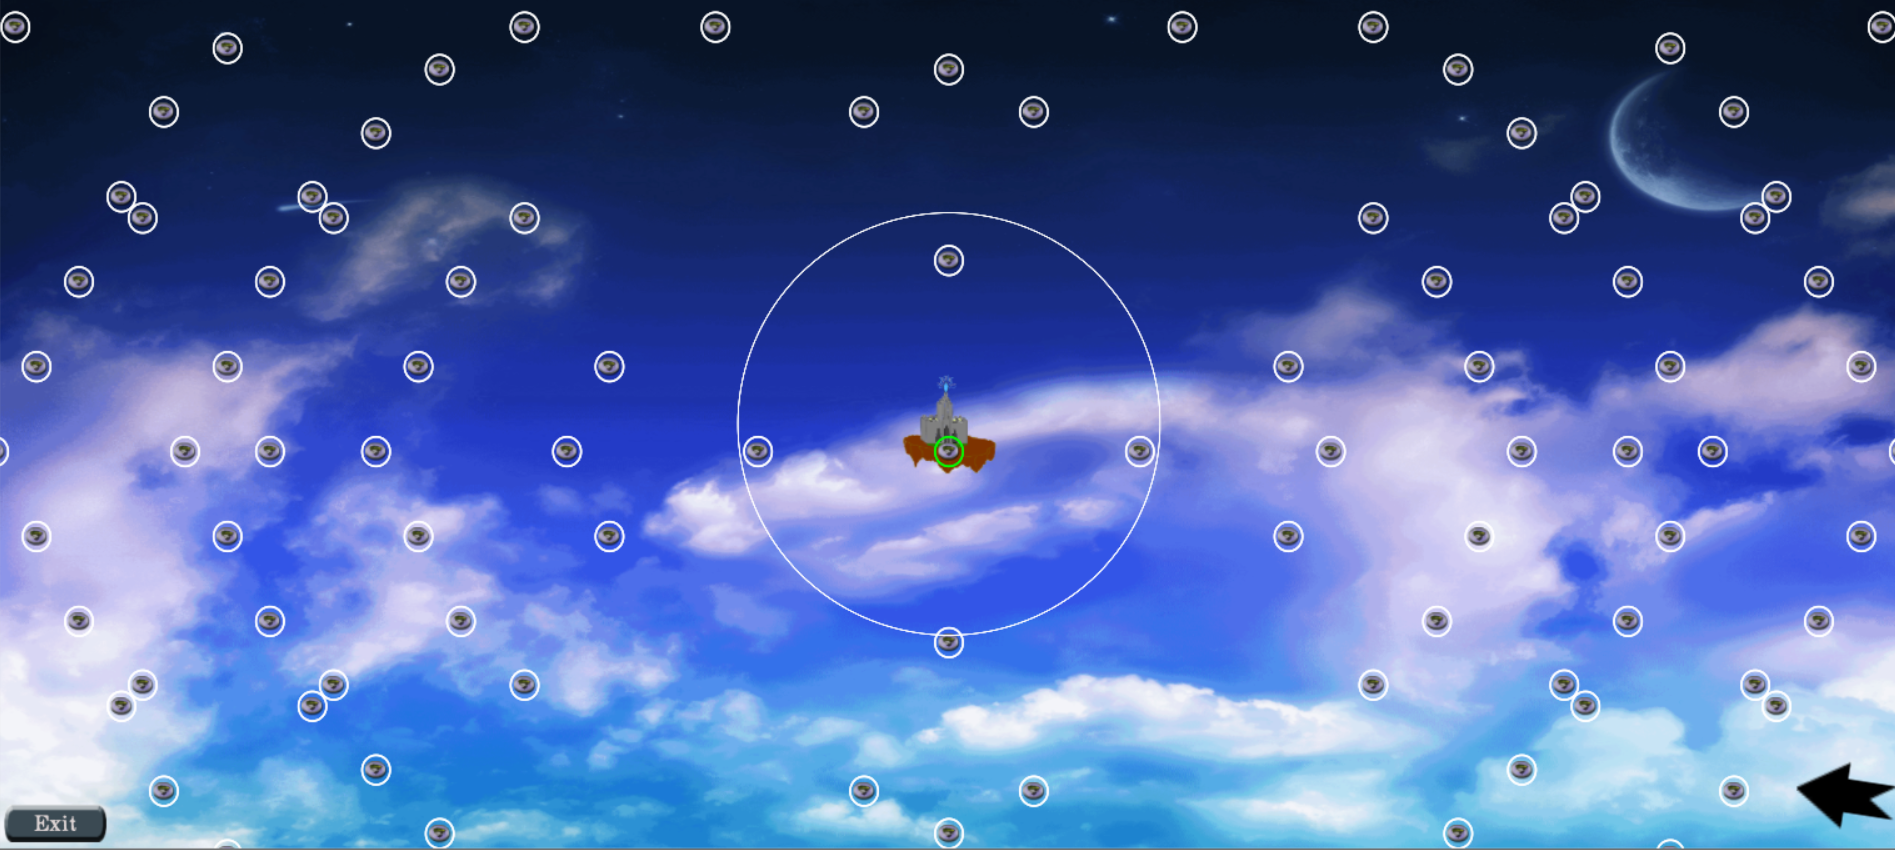
\includegraphics[width=\textwidth]{Images/WorldMapZoom.png}
    \caption{The initial state of the world map centered on teh castle, zoom out to the maximum view.}
    \label{fig:worldmapzoom}
\end{figure}

\subsubsection{Map Layout}
The layout of the map is generated by the use of an L-System (see L-system and the world map section below) and the interpretation rules that comes with it. The main map layout that is being used, has the spreading angle of 30 degrees, though this value vary from the other map layouts that were developed. The map is split up to go in 4 different directions; North, East, South and West. After each island in these directions, the directions spread in 3, one in front, and two to either side in the spreading angle specified. This is the basic pattern that by being repeated, makes up the map.

The pattern's symmetry is visible in figure \ref{fig:worldmapzoom}, where the repeated structure in each of the 4 directions is most visible in the east and west direction.

\subsubsection{Spacing}
Each of the islands that are on the map are placed in a very specific way. They are all spaced so that the distance between them are a little bit less than that of the player-castle's maximum travel distance. This is done to ensure that the players always are able to go to at least \textbf{one} island, no matter where the castle is positioned at any given time. However, because of the use of the L-System, and the fact that the placement pattern is repeating with a set spreading angle, there may be more than one possible destination at a given point in the game. Some of the islands might even be rather close to each other and look like a smaller system of islands. And of course the initial start placing of the castle has 4 islands that are available to be visited, and this is to give the players more freedom of exploration in the game.

\subsubsection{Placement}
The L-system and its rules are there to make sure that the placement of the islands are varied, but at the same time within a given pattern. This means that the look of the map will at times, depending on the how the L-System algorithm is formulated, be able to resemble specific shapes or patterns. Whether this is good or not, depends on how the players respond to it, and if they are even able to see the entirety of the map layout.

\section{PCG - Generating the content}
The purpose of this section is to shed light on the PCG used in the project, what it does and how it does so. First an introduction to the world map generation, which will be followed by the events.
The event generation will first be discussed on a structure level of the variables behind the event, followed by a dissertation of the flavour text generation.

\subsection{L-system and the world map}
\label{sec:lsys}
As described in the background section; the L-System is a way to generate a large outcome based on an axiom and rules on how to change it. With each iteration, the contents of the axiom is changed bit by bit in compliance with the rules that match each element that is being expanded upon.

In our case, we use several other characters than just 'A' and 'B', we add '[', ']', '-' and '+' as well as other letters. The brackets stand for "push" and "pop" respectively, as the map generation have to keep track of positioning, which means we have to introduce a way of saving the current state of the system.

A state as used in the generation of a map layout, has to keep track of positions and angles. So when the L-System hits a '[' in the result string, it knows that it has to save the current state at the current position, as this will be needed when the branching is done and the next ']' is hit. 

When the full expansion of the string is completed, the next stage is to interpret the result. When using this algorithm for a map layout with nodes of different properties, there is a need to use quite a few different characters. For instance, having 'N' will result in a normal node being placed at the current location of the state, whilst having 'E' will result in an end node being placed. Other characters can also be used to have different rules and calculations, e.g. having 'a' and 'A' can result in them having different angles or spacing.
Going through the resulting axiom string, we make a lot of different calculations to be able to properly place the nodes on the map. Every time a node is being placed, the direction is calculated from the state, along with the spacing. Then the algorithm moves the state's "position marker" forward in the calculated direction, and places the correct node at that mark and saves the state along with the location and angling.
This goes on until all characters of the string have been visited, and all the nodes have been placed, then the algorithm is complete.

There are many different patterns that can be made with this algorithm, and in our solution, we made a variety of them, including, but not limited to, star patterns, sea weeds, box fractals and more. 
In the end we are only showcasing the latest and biggest map pattern layout, which is a 4-way branching net of about 500 nodes or islands, that you can visit, as this is a big enough map to be able to generate a large amount of events and outcomes, and as it gives the players a large space to explore.

The map layout itself has a starting node in the center, and expands in 4 directions from there. North, south, east and west, with the initial axiom looking like this: "[N][+++N][---N][------N]". Each of these four directions are also expanding on themselves, with the main rule which is "N" $\rightarrow$ "N[-N][+N][NN]". This means that each node will spawn another to the left, right, and two in the forward direction. The angle is set to be 30 degrees, which means that there will be a good spread of the nodes all across the map. Having set the iteration number to be 3 gives us the number of nodes: 4(initial nodes) * 5(each become 5 new nodes)$\wedge$3(iteration number) + the extra start and goal node $\rightarrow$ 4*5$\wedge$3 + 2 = 502.

\subsection{Event Introduction}
In the next section, you will be introduced to the events of the game. The events are in many aspects the biggest part of the game, as the the physical part of the game, the board game part, is affected by the outcomes of the events. Furthermore the events have special requirements from the board game, and with this the connection between the 2 parts of the game is made.
In the next part of this document, we will go through the events, their structure, how they are constructed and lastly, the flavour text of the events and how they are generated and combined.

\subsection{Events}
\label{sec:eve}
The application's main purpose is to generate events which is the main interaction for the physical part of the game. The events provides resources for players and challenges in form of lost crew or constructed rooms.

Throughout the development of the game there have been several approaches to the problem of generating these events in an interesting manner and ensure the perceived space of possibilities was large enough for the events not to repeat themselves to often.

First the event structure of the final events will be explained. Then a short explanation of the first event generation, detailing where the project began and some of the limitations posed by it. This is followed by an explanation of the final event structure. Finally the how the flavour text is generated is explained.

\subsubsection{Event structure}
In figure \ref{fig:eStruc} you see the general structure of the events in the applications contextual environment. The keywords presented in this structure is referenced in the following subsections in order to specify where the different aspects are being used.

\begin{figure}[!ht]
    \centering
    \includegraphics[scale=0.5]{Images/EventStructure.png}
    \caption{The event structure layout within the application. Each event is tied to a location to on the island in the NodeScene as explained in section \ref{sec:nodeScene}.}
    \label{fig:eStruc}
\end{figure}

Each location in the NodeScene has an event assigned to it. 
Each of these events have two to three event options assigned to them. The options are represented by buttons in the UI in the NodeScene when you explore a location. An option contains the conditions required for resolving the events. 

Each of the event options contains one to three event outcome groups. An event outcome group simply is a bundle of event outcomes. It contains an outcome for each of the result types; success, failure, or neutral. These types are attributed to the outcomes.

Each of the event outcome groups contains three outcomes. An outcome has a type, as explained above, which designates which to pick given if the event is a success, failure, or neutral. The outcome also contains the chance for which this outcome appears. Lastly the outcome contains the pieces and their change amount. 

\subsubsection{Structured Events}
The first implementation focussed on having events for each of the options you could select on the UI. The events were stored in an XML file and loaded with the program. The events were assigned to all the nodes as they were generated.

The general XML structure used for the initial generation can be seen in figure \ref{fig:eGen1}.

\begin{figure}[!ht]
    \centering
    \includegraphics[scale=0.5]{Images/EventGen1.png}
    \caption{This is the first event generation xml layout. If not noted on the arrows, the relationship between the boxes is one to one.}
    \label{fig:eGen1}
\end{figure}

The events were first narrowed down by the type of the event, gathering, research, or diplomacy. The location type were generated at start along with the events. The number of events for each node where selected randomly between one and three.

Next the events were split by the button order, designated as the class, basic for the first button, second for the second button, and third for the third button. 
The classes are, basic, the one which is always present, second, events which have more requirements, and third, events which have more advanced requirements. 

In this early implementation, the conditions, which needed to be fulfilled, were written as text in the \textit{eventText} XML node. The conditions only appeared as text and had no relation to the the game logic. The text was hard coded in file, making each event text broad so it could appear in all contexts.

The event had a list of results, each which had a chance node determining how often the result would appear. When building the event the result is selected using a percentage based selection process. The chance were set between 1 and 100 percent and the total sum of all the results chances were 100. 
Each result had a flavour text associated with it, which was used when resolving the event, and a list of event outcomes. 
The outcomes represented the board pieces and the changes which occurred to them. Each of the outcomes had a piece, the board game piece associated with it, the number range of the amount of pieces given, and extra flavour, which was used for rooms which were destroyed or crew which were injured.

This first structure allowed to populate the application with events which were scripted by the type and selected from a pool of set events. 
However when adding more events, each event needed to be constructed in its entirety each time. This would also means adding or removing pieces would be have to be hard coded directly. 

\subsubsection{Constructed Events}
\label{sec:eventGeneration}
In order to construct a broader range of events, the idea were to have the building blocks to be interchangeable and then generate events from a pool of those blocks to have a greater diversity of the events.

This change were implemented through several iterations, with several changes being made to the algorithms to better suit the game. The final event structure uses an XML file containing building blocks which have a linkage to, and that influences, the general idea of the outcomes of the events.

In figure \ref{fig:eGen2} you can see the total structure of the XML file used in the final event generation algorithm. 
The events are built by selecting a number of conditions and selecting outcomes based on the selected conditions. 
First the conditions and outcomes will be discussed and then how they are combined.

\begin{figure}[!ht]
    \centering
    \includegraphics[scale=0.5]{Images/EventGen2.png}
    \caption{This is the event generation XML structure for the final event generation process. Each box represents an XML node and the writing within the name of the node. The few exceptions to this is if a name has a parentheses around it, then the name in the parentheses is an example of the node names in that level. The figure contains two parts, one for the conditions and one for the outcomes.}
    \label{fig:eGen2}
\end{figure}

The top part of the figure visualizes the structure of a condition. The condition is made up of the piece, the related board piece the players require in order to activate the event option, the amount of pieces required, and the classification type.
The classification type is used in order to group the conditions and limit which pieces appear in what event option, thus ensuring that ordinary pieces are more often in use by the application. There are 3 classification types. Type 0 for required, type 1 for secondary, and type 2 for advanced.

The bottom part of figure \ref{fig:eGen2} is representing the event outcome structure. The events are separated into types like before, gathering and research, and by classes one, two and three. 
The class in this case is the separator for where the different conditions are situated. Class one only contains outcomes which have one condition in total. It is the fall through part of the event structure as the algorithm will populate the events in the end with information.
Class two contains outcomes which have two conditions in total, and also only have events which are made up of conditions type 1 or less. 
This class is used for the secondary options available for the players.
Class three contains outcomes which primarily have two conditions, but where atleast one of these is of type 2.

The outcomes contain the the required conditions, following the rules described above. Each of the conditions have a piece, the board game relation, and the amount of pieces. 
An outcome also contains the results. This node comes in three types; success, failure, and neutral. These nodes have an attribute, denoted in figure \ref{fig:eGen2} with cursive, called chance. This is the outcome's basic chance distribution of the results. 

Each outcome has one or more options attached to it. These basically are the container for the pieces which are influenced by the outcome. If the outcome has more than one option, the one used for event resolution is selected at random. 
By having the options this way, it is possible to add more variety in the outcomes without rewriting the event in any other way.

\subsubsection{Event Generation}
When the events are generated the algorithm is fed two parameters;
the event type, the same as shown in figure \ref{fig:eGen2}, and the number of options the event should have.

For each of the options, the conditions are found and added. The number of conditions added is equal to the option number. The first option having 1 condition, the second one having 2, and the third having 3. 

By design the game requires one of the conditions to be castle crew. In order to accommodate this, the castle crew condition is the only condition which has the type \textit{required}.

The conditions are added by going through the condition list in a randomized order. If the condition found has the type which is less or equal to the current event level, the condition is added. This is done until all the conditions have been added.

The outcomes are filled using the strategy of finding the most complex event which matches the conditions.
This is done by first going through outcomes, of the class related to the option number, in a random order, stopping if the conditions of the outcome matches the conditions in the event. 
If a match is found, the outcome is added to the \textit{EventOption} as an \textit{EventOutcomegroup}. Furthermore the number of conditions used in adding this event - if the event has two conditions; then two events are used - is noted along with the pieces used.

If there is no outcomes which matches the conditions of the event, the algorithm steps down a class, and tries to match with a lower tier. 
This continues until there is no unmatched conditions left.

As a safeguard, the lowest class of outcomes has an entry for each of the possible conditions, ensuring a 1 to 1 match can always occur on the lowest tier. 

The last feature of the event generation is that there only can be one of conditions of a certain type. This is ensured by noting when one such condition is added and not allowing any more to be added after the first.

\subsection{Flavour deconstruction}
\label{sec:flavour}
One of the biggest concerns in terms of being able to present the game with \textit{feel} to the players, was to come up with a way of generating the flavour text. The design choice made was that it would be combined by lesser blocks of text that would be combined into one complete sentence that would display the entirety of the flavour. The way to go about this, was to create dummy data and reverse engineer that into a combination system. First you would create a complete flavour text that would be served as an example. This text would contain a combination the elements that would be wanted in the actual implemented solution; Location types, island names, factions, resources, outcomes, etc.

To exemplify, we will use the dummy flavour "As you arrive at Endriath, you see an old village in the distance. The village seems to have markings that resemble those used by the Highbournes".

The next step would be to reverse engineer this dummy text into blocks of strings that could be combined to reconstruct the original text. So in the start, there is a segment that says "As you arrive at ...". This part would act as an introduction for the island. Next you have the actual name of the island, which is already available in the application. After that there is a smaller part that gives the players insight into what \textit{is} on the island. This segment, however, is split up into 3 pieces; first - "you see ", then "an old village" which is the location type, also available within the application, and lastly " in the distance". After this, the flavour goes on to say something about the location that you are currently at. "The village", again, is available from the application, "seems to have markings that resemble those used by the" - extra flavour made to build mood and a sensation of lore or story, then at the very end is the "Highbournes" which is the faction name of one of the factions saved within the application.

This way of reverse engineering a piece of text leaves us with the pieces: Introduction, Island name, Location introduction, Location type, Location exit, Location Type(again), Mood flavour and Faction name.

After all these blocks has been discovered, the next step is validation. This is done by simply making a set of paper prototypes for each of the pieces, each having a few different possibilities, and then trying to combine them in the same fashion as discovered by the reverse engineering. 

When this all succeeds, the method of combination is discovered and is ready to be implemented into code. Then, when it is all implemented, all that needs to be done is to create a variety of flavours for each of the blocks and the rest will be done by the program.
\subsection{Flavour of the Events}
\label{sec:flav}

The flavour of all the events are split up in smaller blocks that can be combined with other blocks in order to make a complete flavour string. The way they are split up varies from what type of flavour it is.
\subsubsection{The Condition Flavour}
The basic resource blocks, are based on a couple of things. Firstly, each piece has it's own intro part. This part is very basic, and is often no more that one to five words. Secondly, there is an extra block that specifies what the item/room or resource the condition requires, is. After that, there are several other blocks that are organized based upon locations. For instance, the mine will have x amount of flavour texts for each piece, just as the lake will, and all the other locations. This opens up the possibility to quickly come up with new locations, new flavours that will fit that location, and also how the individual pieces can be used there. All flavour blocks are made so that they can be combined together and form one larger and complete flavour text.
\subsubsection{The Introduction Flavour}
The introduction flavour is organized in the same manner as the condition flavour is. However, these are a bit larger pieces of strings that are supposed to give a quick and informative overview of the locations the players are entering. The strings themselves are ordered by event types, i.e. gathering or research, and underneath that, they are ordered by what specific location type it is. Each of the location types can have a multitude of flavour texts, as only one is selected at a time at any given location.
\subsubsection{The Result Flavour}
The result flavour is a bit more comprehensive than the  condition flavour, as it aiming to tell a very short story about each possible result, i.e. alchemy point gained, crew member gained, etc.
Each of these results can have as many flavour texts as wanted, only they have to be written down first. The algorithm will choose one of them for every block that is in the result. And there can be a number of blocks in a result. Yet again, each of these pieces are crafted so that they should be able to be combined with the other pieces that might also be selected, as they each specify their own specific piece.
\subsubsection{The End Flavour}
At the end of the game, there will be displayed a little piece of text telling the players that they made it to the end, and that the game is over. These blocks are not really combinable, as they are meant to be in one string alone.

\subsubsection{General Flavour}
The good thing about having all these pieces of text split up in smaller blocks of strings, is that it allows for many more ways for them to be combined. And adding more flavours will cause few problems, as they all follow the same format and template. It is basically a more structured way of generating larger combinations of text, from smaller pieces of diverse text blocks.

There are a number of different sections used to keep track of all the flavours and data that is being used within the game, and the reason for splitting them up is to better be able to keep track of where one can find what is needed at any given time, without having to go through and search through all its content blindly.
The file used for the structure of the events here is the XML file named "EventStructure". This is the main file where all the smaller blocks of text for all the board pieces, conditions and outcomes are located. It is split up into 7 branches; Conditions, ConditionFlavour, Gathering, Research, IntroFlavour, EndFlavour and ResultFlavour.

The "Conditions" is basically a list of all the possible board pieces that can occur in an event, while the "ConditionsFlavour" is all the flavour associated with those pieces.
"Gathering" and "Research" are holding the event setup, how the events can be combined, what the chances of success, neutral and failure is, and what results options there is for the combinations.
The remaining "IntroFlavour", "EndFlavour" and "ResultFlavour" are holders of the flavour of their respective fields as described above.

\subsection{Combining the flavour text}
The flavour texts are combined in a few ways. Either it is a minor combination of the location name and the owners, Which faction is fighting which faction and where, or the big ones; the conditions and results which will be discussed in more detail here.
\subsubsection{Conditions}
As the event generating algorithm has selected which conditions are to be used in the event, the flavour combination algorithm takes over. What it does, is to have the preset way of combining the flavours and then executing that template on the flavour blocks retrieved from the XML files. Let's create a scenario where there are 2 options to choose from, the first one is a single crew token that is to be sent down, and the second one is to send that crew member and use an alchemy point as well. The location of this scenario will be in a Mine controlled by Humans.
This is how the flavour text would then be combined:

In the first option, the algorithm would open up the XML file called EventStructure.xml, find the place where the condition flavour is located, and load that in. Then the algorithm would go through the branches until it came across the one called "crew". This consists of a basic text and a secondary text. The first part would be "Send", the second would be " x Castle crew". Then it would place the number of crew, in this case 1, between the 2 blocks of flavour, and end up with "Send 1x Castle crew".
Now that we have the introduction of the condition, the next step is to get the location-based flavour. The algorithm would then continue through its data until it came upon the matching location, which in this case would be "mine". Under the mine section, all the pieces are listed again, with their respective lists of flavour blocks. Say the first one is selected, which says: " to explore the mine's riches.". This would then be put at the end of the first part, and combined into the final flavour text for the first option: "Send 1x Castle crew to explore the mine's riches.".

After the first option was completed, the algorithm would see that there was one more to be done, and do the same for that, but since there is more than one piece in that option, the algorithm would do the same as it did for the crew, for the alchemy point.
An example of how the selected text would look like after completion would be this: "Send 1x Castle Crew to explore the mine's riches. Use 1x alchemy point to create a strenght potion for your crew".

On top of having the selection process brought forth from directly accessing the program saves all the previous events that has been made, and that the players have interacted with. So by having access to this information, the algorithm for the events and in turn the flavour texts of these, are able to be made by taking the existing data into account. If an event has had a special occurrence, the outcomes are saved with it and the flavour combining algorithm can then go in to this saved data, take out any important information, and use that as a baseline for the way the new event flavour is generated. Say an event happened, where the players had to use their healing powers to save a person during the exploration of an island, this information would be accessible to the app at a later time. So when the time comes to generate a new event, it can be based on said previous event. For instance; the new event would take place on an island that is controlled by the Highbourne faction, which was the same faction as the previous event, and since the players used their healer on the previous one, the new event could say that now the Highbournes are interested in knowing how the players did that. This opens up for a new set of conditions that the players can be presented with. Basic options like "Show them how it is done" or "Refuse to show them" are just 2 examples. The outcomes can then be modified to for example say that if the players were to help them out, they are rewarded with reputation gains, crystals or what ever they might get. And on the other side, the negative outcome could be something like the Highbournes tries to kill one of the players' crew in hopes that they once again will witness the amazing effects of the players' healing skills.
\subsubsection{Results}
Much in the same way that the condition flavour is combined, the result flavour is also combined. It selects a flavour string for each of the resulting rewards or penalty. To exemplify we will use the results: 2 Building materials and 1 alchemy point gained.
The combination would happen like this:

First the algorithm would go into the XML file and find the part where the building material texts are located. Then it would select one of the available flavours, for instance "Your castle crew scavenged all the possible building material they could find". This string would then be saved and the algorithm would go to the next result and find a flavour for that one as well: "As your crew return, you see that they have some strange alchemical material within their findings". 
These two strings would then be combined into one complete flavour text which would look like this: "Your castle crew scavanged all the possible building material they could find. As your crew return, you see that they have some strange alchemical material within their findings."

Should there be more than these 2 result pieces, the algorithm would go on to do the same combination and add the other blocks to the finalized result flavour.

\section{The app - From start to end}
In this section you will get an overview of how the developed application runs from start to end. 

Each of the states given in section \ref{sec:scen} and which processes that is executed and how will be detailed in the following subsections.
Each of the scenes, all have a controller related to them. This is the main component in the interaction with the visuals and the data in the app. As we go through the states, the stated actions are, unless noted other wise, directly controlled by such a controller.

\subsection{StartMenu}
The game starts in the StartMenu scene. This scene contains visually nothing but a button labelled "StartGame". 
However behind the visuals the application is loading some of the needed data to run a game.

The Datamanager (see section \ref{sec:datman}) is loading information in the background. 
All the board piece information and all the factions, stored in xml files, are loaded and the factions are initialized. 
This data is being used throughout the entire runtime and needs to be readily available.

After all the pieces and factions are in place, the application generates the statistics of all the world nodes, their position, their description, their name, the controlling faction, and all of the statistics for the locations within it.
The only thing which is not being loaded in this instance is the events for each of the locations in the NodeScene (see section \ref{fig:nodescene}). The reason the events are not being loaded stems both from the work load and for saving computing power in the end. As it is very unlikely that the players ever visit every node and see every event, there is no reason to initialize all the events at start-up. 
All the generated nodes are stored and saved in the Datamanager so it can be used throughout the game.

The full explanation of the generation of nodes is detailed in the following section.

The scene changes once the "StartGame" button is pressed, and the "WorldScene" is loaded.

\subsubsection{Generate Nodes}
The nodes are generated when the map structure is being generated using the L-System (see section \ref{sec:lsys} above for the detailed description of how the algorithm works).

A node is generated for each of the corresponding characters in the string generated by the L-system.
The L-system provides the position of the node, along with the type of the node as determined by the character in the string. 
The node is randomly assigned a faction from the available factions stored in the Datamanager. Once the faction is set the node is assigned a name from a list of possible names, and is independently given a description of the location, which incorporates the faction set earlier.

The world node is then assigned two sub nodes which relates to the locations which will be available on the island in the NodeScene. The different nodes have an event type set, one has "gathering" and the other "research".
Each of the nodes are given a name, which is the name of the location, e.g. mine; and a matching description of such a location, both based on the type of event which is tied to the node.

\subsection{World map And World Controller}
The world map in the "WorldScene" is the were the players will move from island to island over the course of the game. 

This scene starts by instantiating the world nodes based on the statistics stored in the Datamanager. As the statistics are kept in the Datamanager, whenever the players return to this scene, the same function is called, taking the changes made by the players into account. 

Once all the nodes are spawned, the controller also spawns the player object at the position which is stored in the Datamanager, initially next to the start node. 
As the player token is spawned, the main camera, which controls the viewport, is centred on the token as well. As the position of the players change during the game, the centering allows the players to quickly find their bearings.

If the players enter this scene, after completing a special event, and they have managed to change their standing with one of the factions in the game, a dialogue box appears, notifying the players of the change.

As the application runs, the camera position and zoom is subject to change 

Whilst in the world map, the players have the possibility of moving the view around and zoom in and out in order to get the overview required.

Whenever an island in the world map is clicked, a dialogue box pops up which contains the name of the island along with a flavour text of the location, both acquired from the world node. 
If the players choose to travel to the location, the player token moves towards the it, ignoring any other collisions, and loads the "NodeScene" when the island and player token collides. 

\subsubsection{WorldPlayer}
The "WorldPlayer" is responsible for moving the player token as long as a target is set. 

It also controls the action to take on collision with the target island. The target of the player is allowed to be a destination which the players have already explored, however, they cannot explore it again. When a target is reached, the controller checks whether it has already been visited, and if so, the players do not load the "NodeScene" as explained above.

The last case is if the target node is the goal node. This will cause the application to load the "ScoreScene" and effectively end the game.
As the "ScoreScene" is loaded, the Datamanager is cleared of all the saved nodes, such that a new game can be started.

\subsection{NodeScene and Generating events}
Once the player has reached an island they have chosen to explore, the NodeController springs to life. 

The controller first generates the location nodes for each of the locations, as set by the L-system.
The events for each of the locations is generated by supplying the type of event and how many event options. The full description of the events is covered in section \ref{sec:eve}.
Once the event is generated, the location sprite is instantiated. Using the name of the location, the sprite related and the location of said sprite is found in a related XML file which keeps a list of all the locations, the name of their sprites, where they should be instantiated, and the scaling factor which should be used.

Exploring one of the nodes opens the event panel which allows the player to explore the event. 

The event is resolved after the players have chosen an option available to them. Once the option have been chosen an outcome of the event is generated.
The final outcome gets a modified chance of success and failure depending on whether the current faction is allied or an enemy. 
The allegiance of the faction also influence the amount of resources rewarded. If the island is controlled by a friendly faction, the player gets the highest possible amount; if the controlling faction is an enemy, the lowest possible amount; and if the faction is neutral a range in between the two.

\subsubsection{Special Events and factions}
If a resolved event is of the \textit{third class}, and there currently is no active special events. The current resolved event is used to begin the special event generation.

Whenever the NodeScene is loaded after a saved event is set as active, a check is made to see how many turns has passed since the activation. Once the amount passes a certain threshold, a special event is activated.

If the special event matches specific criteria then a factional request will come for the players. Else there will be a struggle between to factions, in which the player can choose to intervene.

The special events are the key point of interaction for changing the relationship with each individual faction.

The event can have to different overall configurations.
The first configuration is a battle between two factions, which ask you to pick a side in the conflict and aid against the other.
After a side has been picked, the factional relationship is updated, +100 for the faction you have aided and -100 for the other faction.

The other configuration is more complex

